\problemname{Hubtown}

\noindent
Hubtown is a large Nordic city which is home to $n$ citizens.
Every morning, each of its citizens wants to travel to the central hub from which the city gets its name, by using one of the $m$ commuter trains which pass through the city.
Each train line is a ray (i.e., a line segment which extends infinitely long in one direction), ending at the central hub, which is located at coordinates $(0, 0)$.
However, the train lines have limited capacity (which may vary between train lines), so some train lines may become full, leading to citizens taking their cars instead of commuting.
The city council wishes to minimize the number of people who go by car.  In order to do this, they will issue instructions stating which citizens are allowed to take which train.

A citizen will always take the train line which is of least angular distance from its house.  However, if a citizen is exactly in the middle between two train lines, they are willing to take either of them, and city council can decide which of the two train lines the citizen should use.  See Figure~\ref{fig:hubtown} for an example.

\begin{figure}[!h]
  \centering
  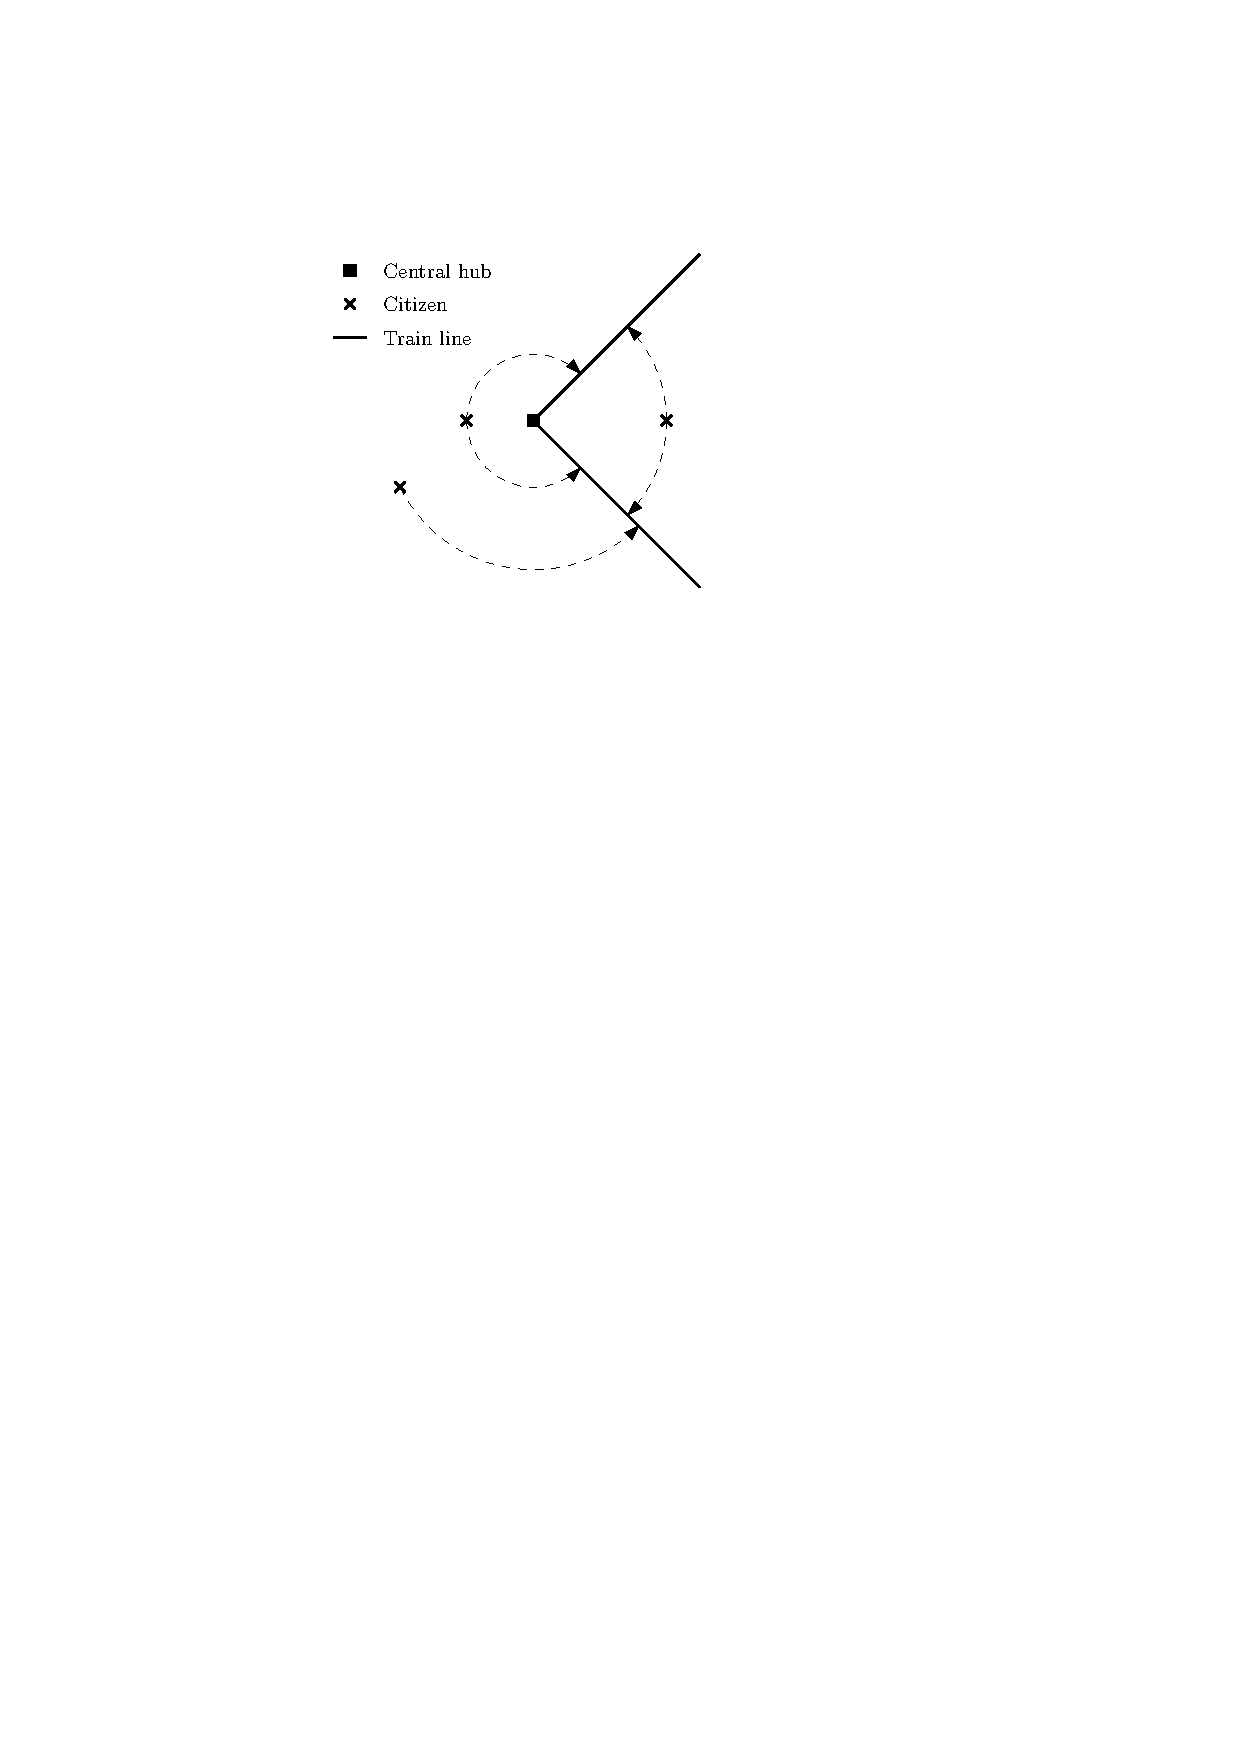
\includegraphics[width=0.31\textwidth]{sample}
  \caption{Illustration of Sample Input 1.  The dashed arrows indicate which train lines the citizens are closest to (note that we are measuring angular distances, not Euclidean distance).}
  \label{fig:hubtown}
\end{figure}

Your task is to help the council, by finding a maximum size subset of citizens who can go by train in the morning to the central hub, ensuring that each of the citizens take one of the lines they are closest to, while not exceeding the capacity of any train line. For this subset, you should also print what train they are to take.

\section*{Input}

The first line of input contains two integers $n$ and $m$, where
$0 \le n \le 200\,000$ is the number of citizens, and $1 \le m \le
200\,000$ is the number of train lines.

The next $n$ lines each contain two integers $x$ and $y$, the
Cartesian coordinates of a citizen's home.  No citizen lives at the
central hub of the city.

Then follow $m$ lines, each containing three integers $x$, $y$, and $c$ describing a train line, where $(x, y)$ are the
coordinates of a single point (distinct from the central hub of the
city) which the train line passes through and $0 \le c \le n$ is the
capacity of the train line.  The train line is the ray
starting at $(0, 0)$ and passing through $(x, y)$.

All coordinates $x$ and $y$ (both citizens' homes and the points defining the train lines) are bounded by $1000$ in absolute value.
No two train lines overlap, but multiple citizens may live at the same coordinates.

\section*{Output}

First, output a single integer $s$ -- the maximum number of citizens who can go by train.
Then, output $s$ lines, one for each citizen that goes by train.
On each line, output the index of the citizen followed by the index of the train line the citizen takes.
The citizens are numbered from $0$ to $n-1$ in the order they are given in the input.  The trains are numbered from $0$ to $m-1$ in the order they are given in the input.   The output lines may be given in any order.
